% !TEX root = ../../presentation.tex

\begin{slide}{Layer Layer}
\only<1>{
\begin{tikzpicture}[thick]
  \tikzset{box/.style={draw, rectangle, text width=1.75cm, text height=0.75cm}}

  % Model
  \path (0, 0) coordinate (z) node {$\mathbf{z}$};
  \path (1.75, 0) coordinate [box] (G) node {Generator};
  \path (4.25, -0.8) coordinate (f)
        node {
\includegraphics[scale=0.1]{cppcon-logo-blurry}};
  \path (4.25, +0.8) coordinate (r)
        node {
\includegraphics[scale=0.1]{cppcon-logo}};
  \path (7.25, 0) coordinate [box, text width=2.2cm] (D) node {Discriminator};
  \path (5.45, 0) coordinate (_);
  \path (9.75, 0) coordinate (P) node {$\mathbf{P(\text{real})}$};

  % Edges
  \draw [->, shorten <=0.25cm] (z) -- (G);
  \draw [->, shorten >=0.7cm] (G) -- (f);
  \draw [shorten <=0.775cm] (f) -- (_);
  \draw [shorten <=0.75cm] (r) -- (_);
  \draw [->] (_) -- (D);
  \draw [->, shorten >=0.75cm] (D) -- (P);
\end{tikzpicture}
}

\only<2>{
\begin{tikzpicture}[thick]
  \tikzset{box/.style={draw, rectangle, text width=3cm, text height=1cm}}

  % Model
  \path (0, 0) coordinate (r)
        node {
\includegraphics[scale=0.1]{cppcon-logo}};
  \path (4, 0) coordinate [box] (D) node {Discriminator};
  \path (8, 0) coordinate (P) node {$\mathbf{P(\text{real})}$};

  % Edges;
  \draw [->, shorten <=0.75cm] (r) -- (D);
  \draw [->, shorten >=0.75cm] (D) -- (P);
\end{tikzpicture}
}

\only<3>{
\begin{tikzpicture}[thick]
  \tikzset{box/.style={draw, rectangle, text width=3cm, text height=1cm}}

  % Model
  \path (0, 0) coordinate (r)
        node {
\includegraphics[scale=0.1]{cppcon-logo}};

  \foreach \x/\l in {0/Convolution,%
                     1/Convolution,%
                     2/Convolution,%
                     3/Convolution,%
                     4/Flatten,%
                     5/Dense%
                     } {
    \draw ({1.75 + \x * 0.8}, -1.25) rectangle ++(0.6, 2.5)
          node [midway, rotate=90] {\l};

  }
  \path (8, 0) coordinate (P) node {$\mathbf{P(\text{real})}$};

  % Edges;
  \draw [->, shorten <=0.75cm] (r) -- (1.75, 0);
  \draw [->, shorten >=0.75cm] (6.35, 0) -- (P);
\end{tikzpicture}
}
\end{slide}

% \begin{slide}{Layers: Dense}
% \begin{tikzpicture}
%   \tikzset{neuron/.style={draw, circle, thick, inner sep = 7pt}};
%
%   % Input layer
%   \foreach \i in {0, ..., 3} {
%     \path (0, {-\i}) coordinate [neuron] (x\i) node {$x_\i$};
%   }
%   \draw (0, -3.8) node {\textbf{Input Layer}};
%
%   % Output layer
%   \foreach \i in {0, ..., 3} {
%     \path (3, {-\i}) coordinate [neuron] (y\i) node {$y_\i$};
%   }
%   \draw (3, -3.8) node {\textbf{Output Layer}};
%
%   % Dimensions
%   \only<5-> {
%     \draw [Red, semithick, <->] (-0.8, -3.2) -- ++(0, 3.3) node [midway, left] {$k$};
%     \draw [NavyBlue, semithick, <->] (4, -3.2) -- ++(0, 3.3) node [midway, right] {$l$};
%   }
%
%   % Connections
%   \onslide<2->{
%     \foreach \i in {0, ..., 3} {
%       \foreach \j in {0, ..., 3} {
%         \ifnum\i=0
%           \draw [semithick, ->] (x\i) -- (y\j);
%         \else
%           \onslide<4-> {
%             \draw [semithick, ->] (x\i) -- (y\j);
%           }
%         \fi
%       }
%       \ifnum\i=0
%         \onslide<3>{
%           \draw [line width=0] (x0) -- (y0)
%                 node [above, midway] {$w_{0,0}$};
%
%           \draw [line width=0] (x0) -- (y1)
%                 node [above, pos=0.55, rotate=-10] {$w_{0,1}$};
%
%           \draw [line width=0] (x0) -- (y2)
%                 node [above, pos=0.65, rotate=-20] {$w_{0,2}$};
%
%           \draw [line width=0] (x0) -- (y3)
%                 node [above, pos=0.7, rotate=-30] {$w_{0,3}$};
%         }
%       \fi
%     }
%   }
% \end{tikzpicture}
%
% \vspace{0.3cm}
% \only<5->{
%   \begin{tikzpicture}[semithick]
%     % Matrices
%     \draw (0, 0) node {
%       \scalebox{0.75}{
%       $
%       \begin{bmatrix}
%         x_{0,0} & x_{0,1} & x_{0,2} & x_{0,3}  \\
%         x_{1,0} & x_{1,1} & x_{1,2} & x_{1,3}  \\
%         \vdots & \vdots & \vdots & \vdots      \\
%         x_{n,0} & x_{n,1} & x_{n,2} & x_{n,3}  \\
%       \end{bmatrix}
%       %
%       \times
%       %
%       \begin{bmatrix}
%         w_{0,0} & w_{0,1} & w_{0,2} & w_{0,3} \\
%         w_{1,0} & w_{1,1} & w_{1,2} & w_{1,3} \\
%         w_{2,0} & w_{2,1} & w_{2,2} & w_{2,3} \\
%         w_{3,0} & w_{3,1} & w_{3,2} & w_{3,3} \\
%       \end{bmatrix}
%       %
%       =
%       %
%       \begin{bmatrix}
%         y_{0,0} & y_{0,1} & y_{0,2} & y_{0,3}  \\
%         y_{1,0} & y_{1,1} & y_{1,2} & y_{1,3}  \\
%         \vdots & \vdots & \vdots & \vdots      \\
%         y_{n,0} & y_{n,1} & y_{n,2} & y_{n,3}  \\
%       \end{bmatrix}
%       $
%       }
%     };
%
%     % Labels
%     \draw [<->] (-5.15, -0.77) -- ++(0, 1.54) node [midway, left] {$n$};
%     \draw [Red, <->] (-4.9, 0.95) -- ++(2.8, 0) node [midway, above] {$k$};
%     \draw [NavyBlue, <->] (-1.4, 0.9) -- ++(2.8, 0) node [midway, above] {$l$};
%   \end{tikzpicture}
% }
% \end{slide}
%
% \begin{slide}{Layers: Dense}
% \begin{tikzpicture}
%   \tikzset{neuron/.style={draw, circle, thick, inner sep = 7pt}};
%
%   % Input Layer
%   \foreach \y/\l in {0/0, 1/1, 2/2, 4/l} {
%     \path (0, {-\y * 0.9}) coordinate [neuron] (x\l)
%           node {\hspace{0.5mm}\footnotesize$x_{\l}$};
%   }
%   % Label
%   \draw (0, -4.4) node {\textbf{Pixels}};
%
%   \draw (0, -2.55) node {\LARGE$\vdots$};
%
%   % Output Layer
%   \path (3, -1.5) coordinate [neuron, inner sep=7pt] (P)
%         node {\hspace{0.4mm}\footnotesize$P$};
%   % Label
%   \draw (4.7, -1.52) node {\textbf{Probability}};
%
%   % Edges
%   \foreach \i in {0, 1, 2, l} {
%     \draw [semithick, ->] (x\i) -- (P);
%   }
% \end{tikzpicture}
% \end{slide}

\begin{slide}{Layers: Convolution}
  \begin{tikzpicture}[semithick]
    % Image
    \draw (0, 0) grid ++(3, 3);

    % Grayscale pixel values
    \only<1>{
      \foreach \x in {0, ..., 2} {
        \foreach \y in {0, ..., 2} {
          \randomgray
          \fill [ultra thin, randomgray] (\x, \y) rectangle ++(1, 1);
        }
      }
    }

    \only<2-3>{
    \draw (0.5, 0.5) node {$0.8$};
    \draw (1.5, 0.5) node {$0.3$};
    \draw (2.5, 0.5) node {$0.5$};
    \draw (0.5, 1.5) node {$0.7$};
    \draw (1.5, 1.5) node {$0.2$};
    \draw (2.5, 1.5) node {$0.6$};
    \draw (0.5, 2.5) node {$0.4$};
    \draw (1.5, 2.5) node {$0.9$};
    \draw (2.5, 2.5) node {$0.1$};
    }

    \draw (1.5, -0.5) node {Image};

    \only<3-3>{
    \draw (4, 0) grid ++(2, 2);

    \draw (4.5, 0.5) node {$3.1$};
    \draw (5.5, 0.5) node {$0.9$};
    \draw (4.5, 1.5) node {$5.7$};
    \draw (5.5, 1.5) node {$2.4$};

    \draw (5, -0.48) node {Kernel};
    }

    \only<4-5>{
      \draw (0.5, 0.5) node {$0.8$};
      \draw (1.5, 0.5) node {$0.3$};
      \draw (2.5, 0.5) node {$0.5$};
      \draw (0.5, 1.5) node {\tiny$3.1 \cdot 0.7$};
      \draw (1.5, 1.5) node {\tiny$0.9 \cdot 0.2$};
      \draw (2.5, 1.5) node {$0.6$};
      \draw (0.5, 2.5) node {\tiny$5.7 \cdot 0.4$};
      \draw (1.5, 2.5) node {\tiny$2.4 \cdot 0.9$};
      \draw (2.5, 2.5) node {$0.1$};

      \draw [red] (0, 1) grid (2, 3);
    }
    \only<5-> {
      \draw [red] (4, 1) rectangle ++(1, 1) node [midway, black] {$6.79$};
      \draw (5, -0.5) node {Output};
    }
    \only<6-7>{
    \draw (0.5, 0.5) node {$0.8$};
    \draw (1.5, 0.5) node {$0.3$};
    \draw (2.5, 0.5) node {$0.5$};
    \draw (0.5, 1.5) node {$0.7$};
    \draw (1.5, 1.5) node {\tiny$3.1 \cdot 0.2$};
    \draw (2.5, 1.5) node {\tiny$0.9 \cdot 0.6$};
    \draw (0.5, 2.5) node {$0.4$};
    \draw (1.5, 2.5) node {\tiny$5.7 \cdot 0.9$};
    \draw (2.5, 2.5) node {\tiny$2.4 \cdot 0.1$};

      \draw [NavyBlue] (1, 1) grid (3, 3);
    }
    \only<7-> {
      \draw [NavyBlue] (5, 1) rectangle ++(1, 1) node [black, midway] {$6.53$};
    }
    \only<8-9>{
    \draw (0.5, 0.5) node {\tiny$3.1 \cdot 0.8$};
    \draw (1.5, 0.5) node {\tiny$0.9 \cdot 0.3$};
    \draw (2.5, 0.5) node {$0.5$};
    \draw (0.5, 1.5) node {\tiny$5.7 \cdot 0.7$};
    \draw (1.5, 1.5) node {\tiny$2.4 \cdot 0.2$};
    \draw (2.5, 1.5) node {$0.6$};
    \draw (0.5, 2.5) node {$0.4$};
    \draw (1.5, 2.5) node {$0.9$};
    \draw (2.5, 2.5) node {$0.1$};

      \draw [Green] (0, 0) grid (2, 2);
    }
    \only<9-> {
      \draw [Green] (4, 0) rectangle ++(1, 1) node [black, midway] {$7.67$};
    }
    \only<10-11>{
    \draw (0.5, 0.5) node {$0.8$};
    \draw (1.5, 0.5) node {\tiny$3.1 \cdot 0.3$};
    \draw (2.5, 0.5) node {\tiny$0.9 \cdot 0.5$};
    \draw (0.5, 1.5) node {$0.7$};
    \draw (1.5, 1.5) node {\tiny$5.7 \cdot 0.2$};
    \draw (2.5, 1.5) node {\tiny$2.4 \cdot 0.6$};
    \draw (0.5, 2.5) node {$0.4$};
    \draw (1.5, 2.5) node {$0.9$};
    \draw (2.5, 2.5) node {$0.1$};

      \draw [Magenta] (1, 0) grid (3, 2);
    }
    \only<11-> {
      \draw [Magenta] (5, 0) rectangle ++(1, 1) node [black, midway] {$3.96$};
    }
  \end{tikzpicture}
\end{slide}

\begin{slide}{Layers: Convolution}
  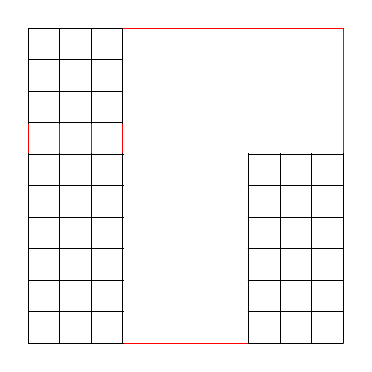
\begin{tikzpicture}
    % R layer (feature map)
    \yzplane{0}{
      \draw [NavyBlue] (0, 0) rectangle ++(4, 4);
    }
    \xyplane{4}{
      \draw [NavyBlue] (0, 0) rectangle ++(0.4, 4);
    }
    \xzplane{0}{
      \draw [NavyBlue] (0, 0) rectangle ++(0.4, 4);
    }
    \xzplane{4}{
      \draw [NavyBlue] (0, 0) rectangle ++(0.4, 4);
    }

    % G layer (feature map)
    \yzplane{0.4}{
      \draw [Green] (0, 0) rectangle ++(4, 4);
    }
    \xyplane{0}{
      \draw [Green] (0.4, 0) rectangle ++(0.4, 4);
    }
    \xyplane{4}{
      \draw [Green] (0.4, 0) rectangle ++(0.4, 4);
    }
    \xzplane{0}{
      \draw [Green] (0.4, 0) rectangle ++(0.4, 4);
    }
    \xzplane{4}{
      \draw [Green] (0.4, 0) rectangle ++(0.4, 4);
    }

    % B layer (feature map)
    \yzplane{0.8}{
      \draw [Red] (0, 0) rectangle ++(4, 4);
    }
    \xyplane{0}{
      \draw [Red] (0.8, 0) rectangle ++(0.4, 4);
    }
    \xyplane{4}{
      \draw [Red] (0.8, 0) rectangle ++(0.4, 4);
    }
    \xzplane{0}{
      \draw [Red] (0.8, 0) rectangle ++(0.4, 4);
    }
    \xzplane{4}{
      \draw [Red] (0.8, 0) rectangle ++(0.4, 4);
    }

    \foreach \i/\j in {0/1, 0.4/2, 0.8/3, 1.2/4} {
    \only<\j>{
      \xyplane{\i}{
        \draw (0, 2.79) grid [step=0.4] ++(1.2, 1.21);
      }
      \xyplane{{\i+1.2}}{
        \draw (0, 2.79) grid [step=0.4] ++(1.2, 1.21);
      }
      \yzplane{0}{
        \draw (2.79, \i) grid [step=0.4] ++(1.21, 1.21);
      }
      \yzplane{1.2}{
        \draw (2.79, \i) grid [step=0.4] ++(1.21, 1.21);
      }
      \xzplane{4}{
        \draw (0, \i) grid [step=0.4] ++(1.21, 1.21);
      }
      \xzplane{2.8}{
        \draw (0, \i) grid [step=0.4] ++(1.21, 1.21);
      }
    }
    }
  \end{tikzpicture}
\end{slide}

\begin{slide}{Layers: Convolution}
  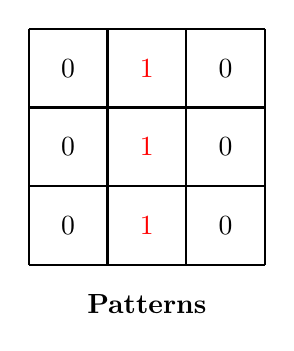
\begin{tikzpicture}[thick]
    \draw (0, 0) grid ++(3, 3);
    \foreach \i in {0, ..., 2} {
      \foreach \j in {0, ..., 2} {
        \ifnum\i=1
          \draw ({\i+0.5}, {\j+0.5}) node {\color{Red}1};
        \else
          \draw ({\i+0.5}, {\j+0.5}) node {0};
        \fi
      }
    }

    \onslide<2->{\draw (1.5, -0.5) node {\textbf{Patterns}};}
  \end{tikzpicture}
  \hspace{2cm}
  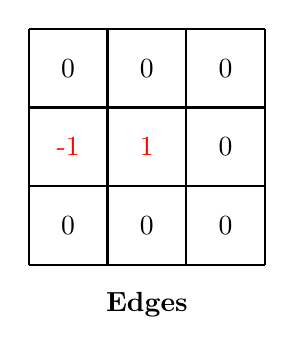
\begin{tikzpicture}[thick]
    \draw (0, 0) grid ++(3, 3);
    \foreach \i in {0, ..., 2} {
      \foreach \j in {0, ..., 2} {
        \ifnum\j=1
          \ifnum\i=0
            \draw ({\i+0.5}, {\j+0.5}) node {\color{Red}-1};
          \else
            \ifnum\i=1
              \draw ({\i+0.5}, {\j+0.5}) node {\color{Red}1};
            \else
              \draw ({\i+0.5}, {\j+0.5}) node {0};
            \fi
          \fi
        \else
          \draw ({\i+0.5}, {\j+0.5}) node {0};
        \fi
      }
    }

    \onslide<3->{\draw (1.5, -0.5) node {\textbf{Edges}};}
  \end{tikzpicture}
\end{slide}

% \begin{slide}{Layers: Convolution}
%   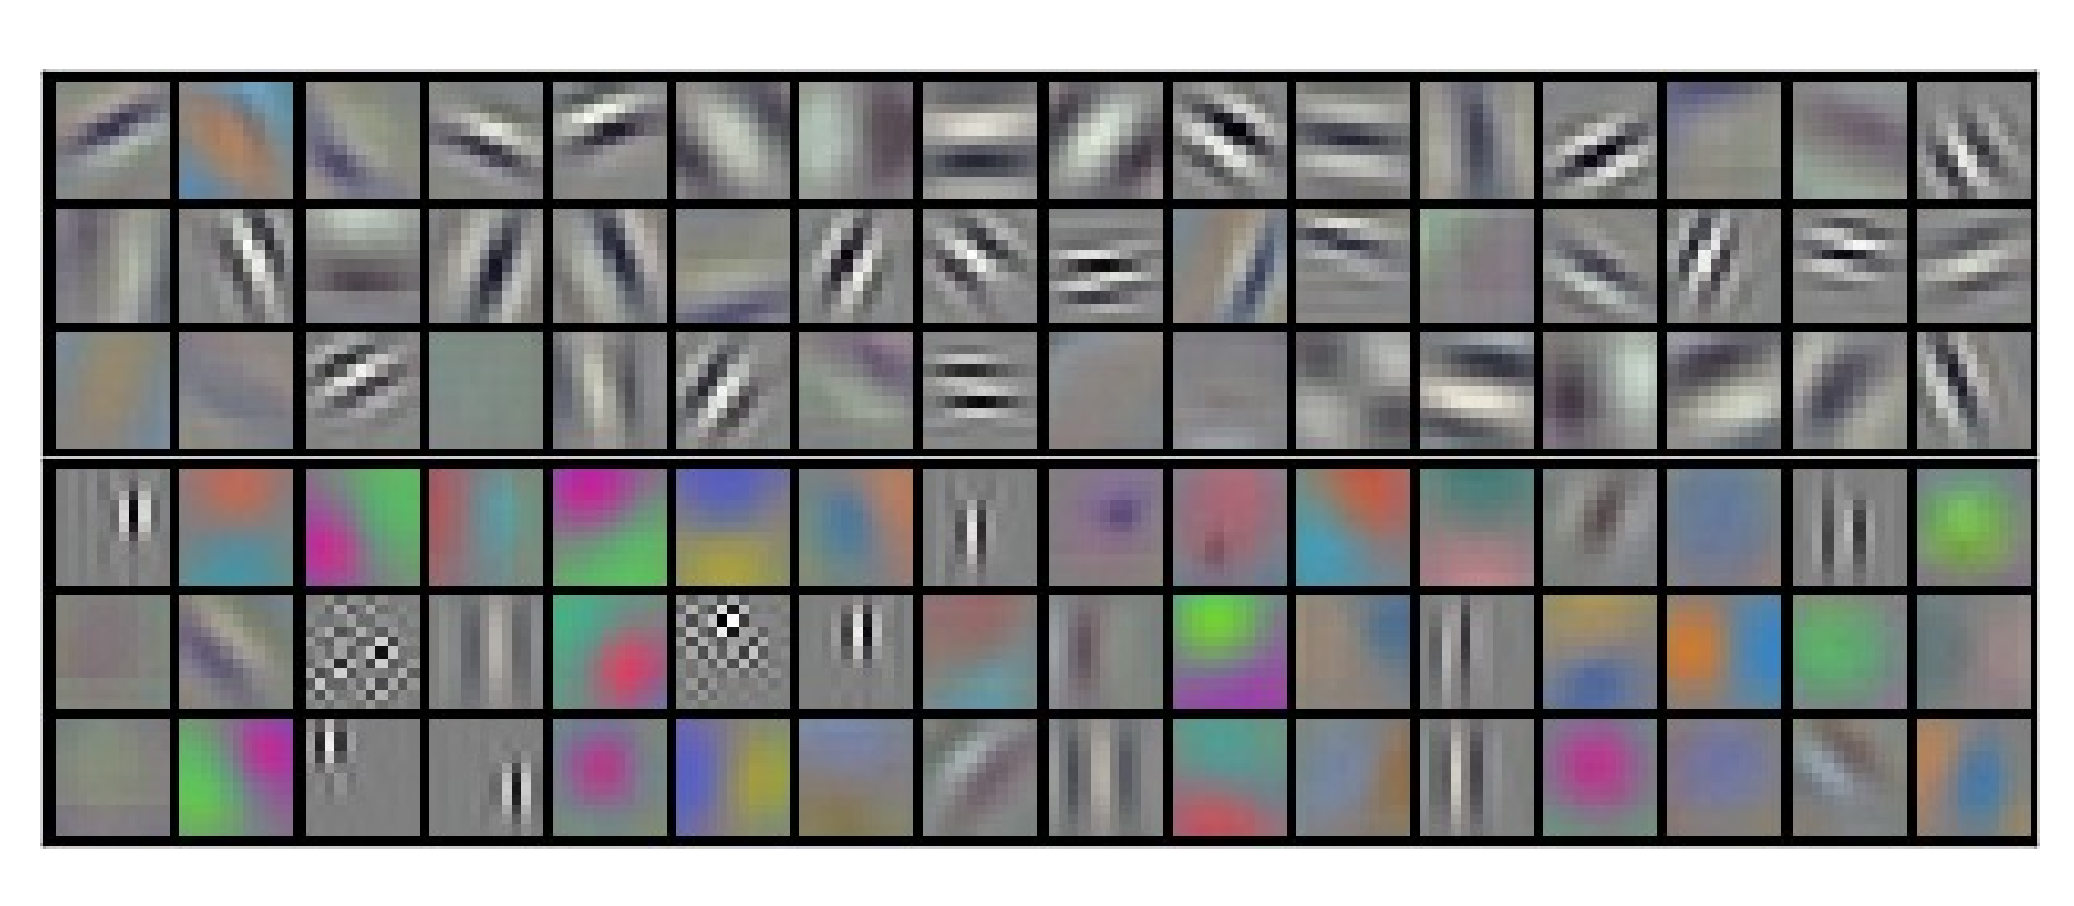
\includegraphics[scale=0.275]{alexnet-kernels}
%
%   \scriptsize
%   AlexNet: Krizhevsky et al. (2012)
% \end{slide}

% \begin{slide}{Layer: Convolution}
% % Stride 1
% \begin{tikzpicture}[semithick]
%     % Full grid
%     \draw (0, 0) grid [step=0.5] (2, 2);
%
%     \newcount\slidecount\relax
%     \slidecount=1\relax
%     \foreach \y in {1, 0.5, 0} {
%       \foreach \x in {0, 0.5, 1} {
%         \only<\the\slidecount>{
%           \fill [red] (\x, \y) rectangle ++(1, 1);
%           % Draw over
%           \draw (\x, \y) grid [step=0.5] ++(1, 1);
%         }
%         \onslide<\the\slidecount->{
%           \draw [black, fill=red] ({3+\x}, {\y+0.25}) rectangle ++(0.5, 0.5);
%         }
%         \global\advance\slidecount by 1\relax
%       }
%     }
%
%     % Label
%     \draw (1, -0.4) node {\textbf{Stride 1}};
% \end{tikzpicture}
%
% \vspace{0.75cm}
%
% % Stride 2
% \begin{tikzpicture}[semithick]
%     % Full grid
%     \draw (0, 0) grid [step=0.5] (2, 2);
%
%     \newcount\slidecount\relax
%     \slidecount=10\relax
%     \foreach \y in {1, 0} {
%       \foreach \x in {0, 1} {
%         \only<\the\slidecount>{
%           \fill [red] (\x, \y) rectangle ++(1, 1);
%           % Draw over
%           \draw (\x, \y) grid [step=0.5] ++(1, 1);
%         }
%         \onslide<\the\slidecount->{
%           \draw [black, fill=red]
%                 ({3.25+\x/2}, {\y/2+0.5}) rectangle ++(0.5, 0.5);
%         }
%         \global\advance\slidecount by 1\relax
%       }
%     }
%
%     % Label
%     \draw (1, -0.4) node {\textbf{Stride 2}};
%
%     % Spacer
%     \draw (4.4, 0);
% \end{tikzpicture}
% \end{slide}
%
% \begin{slide}{Layer: Convolution}
% \begin{tikzpicture}[thick]
%   \tikzset{box/.style={draw, rectangle, text width=3cm, text height=1cm}}
%
%   % Model
%   \path (0, 0) coordinate (r)
%         node {
\includegraphics[scale=0.1]{cppcon-logo}};
%   \draw (r)+(0, -1.1) node {\footnotesize\texttt{128 $\times$\hspace{-1mm} 128 \hspace{-1mm}$\times$\hspace{-1mm} 3}};
%
%   \foreach \x/\l/\s\b in {0/Convolution/64$\times$64$\times$32/0,%
%                      1/Convolution/32$\times$32$\times$16/1,%
%                      2/Convolution/16$\times$16$\times$8/0,%
%                      3/Convolution/8$\times$8$\times$4/1,%
%                      4/Flatten/256/0,%
%                      5/Dense/1/0%
%                      } {
%     \draw ({1.75 + \x * 0.8}, -1.25) rectangle ++(0.6, 2.5)
%           node [midway, rotate=90] {\l};
%     \ifnum\b=0
%       \draw ({2 + \x * 0.82}, -1.5) node {\tiny\texttt{\s}};
%     \else
%       \draw ({2 + \x * 0.82}, -1.8) node {\tiny\texttt{\s}};
%     \fi
%
%   }
%   \path (8, 0) coordinate (P) node {$\mathbf{P(\text{real})}$};
%
%   % Edges;
%   \draw [->, shorten <=0.75cm] (r) -- (1.75, 0);
%   \draw [->, shorten >=0.75cm] (6.35, 0) -- (P);
% \end{tikzpicture}
%
% \vspace{1cm}
%
% \begin{tabular}{l l}
%   \textbf{Kernel: } & 5 $\times$ 5 \\
%   \textbf{Stride: } & 2
% \end{tabular}
% \end{slide}
